\chapter{Scan}\label{ch:scan}
In order to be able to handle a dynamically changing environment,
we decided to use IR distance sensors,
to check if the map matches the real physical environment.
Initially, our robot is supposed to find the 
shortest path from A to B, on a map.

In rescue situations the map provided does not necessarily match 
the actual environment.
External factors could for example have collapsed walls,
thus obstructing movement.

By using 8 IR sensors, we can detect changes in all directions 
the robot can move in. If a change is detected, this will be
accounted for in the maphandling code,
as explained in Chapter \ref{ch:map_handling}.

\newpage
\section{Sensor}\label{sec:sensor}
For detecting any changes in the layout of the map, we have used analog IR 
sensors. Initially, our idea was to use digital sensors, which would have been 
easier to use, but none were available for testing and implementing. Instead, 
we have used analog sensors, which were available at the university. Having the 
chance to implement and test them earlier during the project, we decided to go 
with them. 
Figure \ref{fig:sensor} shows the sensors used.

\begin{figure}[htp]
	\centering
	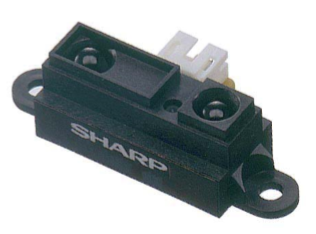
\includegraphics[width=0.2\textwidth]{figures/scan/Sensor.png}
	\caption{Sharp IR GP2Y0A21}
	\label{fig:sensor}
\end{figure}
%
To be able to interpret the voltage received from the sensor, we referred 
to the datasheet of the sensor. Figure \ref{fig:distance_voltage} shows
the approximate voltage output of the sensors in respect to the distance measured.
Voltage values below 10cm should be overlooked since the sensor is not able
to detect distances closer than 10cm.

\begin{figure}[htp]
	\centering
	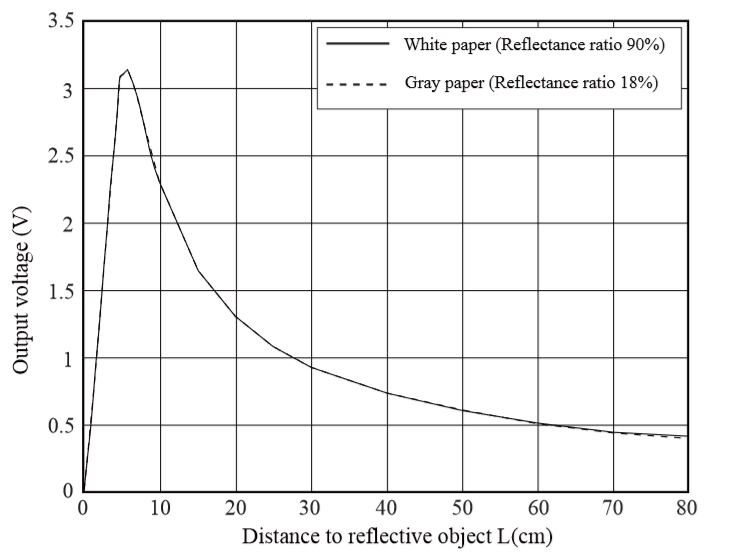
\includegraphics[width=0.7\textwidth]{figures/scan/OutputVoltage.png}
	\caption{Voltage in respect to Distance}
	\label{fig:distance_voltage}
\end{figure}
\newpage
\section{Scanning}\label{sec:scanning}

The sensors are able do detect distances up to 80 cm. The grid size is 
defined in such manner that it should be able to fit the robot in one square. 
Additionally, the sensors should also be able to detect walls or corners in 
any of the eight directions.
Figure \ref{fig:robot} represents the robot and the range of the sensors relative
to the grid size.

\begin{figure}[htp]
	\centering
	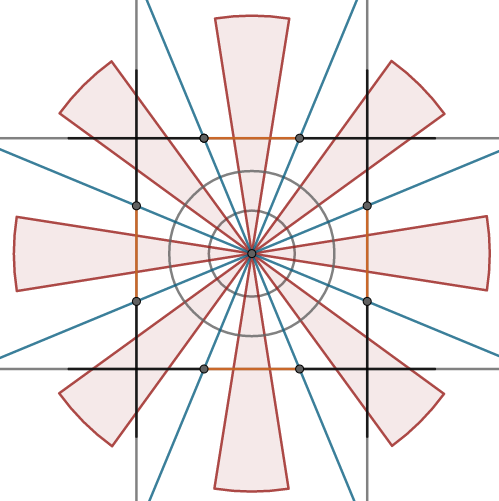
\includegraphics[width=0.4\textwidth]{figures/scan/RangeCalc.png}
	\caption{Robot and Sensor Range}
	\label{fig:robot}
\end{figure}
\begin{table}[htp]
	\centering
	\caption{Color Explanation for Figure \ref{fig:robot}}
	\label{tab:color_explanation}
	\begin{tabular}{|c|c|l|l|l|l|l|l|}
		\hline
		Color  & \multicolumn{7}{c|}{Meaning}                     \\ \hline
		Blue   & \multicolumn{7}{c|}{Limits of Walls and Corners} \\ \hline
		Black  & \multicolumn{7}{c|}{Corner}                      \\ \hline
		Orange & \multicolumn{7}{c|}{Wall}                        \\ \hline
		Red    & \multicolumn{7}{c|}{Range of IR Sensors}         \\ \hline
	\end{tabular}
\end{table}
The {\tt scan} function detects changes, and returns a byte with the observed walls. If the byte returned
matches the one stored in the map, the robot continues on its predefined path.
Otherwise, the byte given by the {\tt scan} function overwrites the one stored in the map
and the robot recalculates the shortest path based on the updated map.
An example of what a byte stored and a byte scanned might look like is given in
Table \ref{tab:scanned_byte}.
 
\begin{table}[htp]
	\centering
	\caption{Map Byte and Scanned Byte}
	\label{tab:scanned_byte}
	\begin{tabular}{|l|*{8}{m{1cm}|}|l|}
	\hline
	Directions & NW & SW & SE & NE & W & S & E & N & Byte	\\ \hline
	Map Byte   & 1  & 0  				  & 0  & 1  				 & 1 & 1 & 1 & 0 & 0x9E    	\\ \hline
	Scan Byte  & 1  & \textcolor{red}{1}  & 0  & \textcolor{red}{0}  & 1 & 1 & 1 & 0 & 0xCE 	   	\\ \hline
	\end{tabular}
\end{table}

\newpage
\section{Implementation}\label{sec:scan_implementation}
The IR sensor was tested on an Arduino Uno. Listing \ref{lst:sensor} 
represents the code to test the sensor, and can also be seen in 
\ref{app:scan}.

\lstinputlisting
[firstline=1,
firstnumber=1,
lastline=28,		
label=lst:sensor,
caption={Sensor Tesing}
]{code/scan/scan.ino}

The value read from the sensor, is multiplied with the value given by
dividing the supply voltage with the ADC resolution, as shown in line 11.
Afterwards, line 13 determines the distance.
Lastly, the value is checked and a boolean value is returned.
\clearpage
Figure \ref{fig:arduino_values} represents the values returned by the
distance sensor.

\begin{figure}[htp]
	\centering
	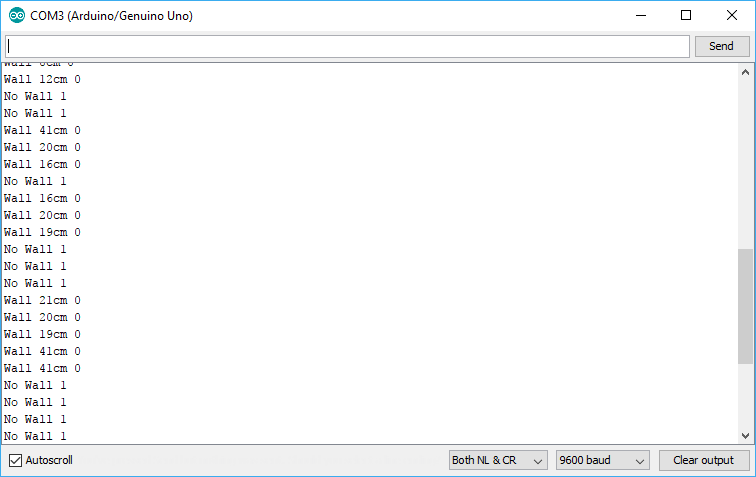
\includegraphics[width=\textwidth]{figures/scan/SerialCom.png}
	\caption{Returned Values}
	\label{fig:arduino_values}
\end{figure}